\textbf{An introduction to organizing peer learning experiences}

\subsection{From syllabus and curriculum to personal and peer learning
plans}

Part of the effectiveness of peeragogy is that the ``syllabus'' or
``curriculum'' -- more generally, the learning plan -- is developed by
the people doing the learning. You don't faint with shock when you see
the reading list if you helped write it.

In peer learning, having a personal learning plan at the outset helps
each participant identify his or her unique learning and teaching
proclivities and capabilities, and effectively apply them in the peer
setting. In developing your personal plan, you can ask yourself the
following questions:

\begin{enumerate}
\item
  What do I most need to learn about in the time ahead?
\item
  What are the best ways I learn, what learning activities will meet my
  learning needs, what help will I need and how long will it take?
\item
  What will I put into my personal portfolio to demonstrate my learning
  progress and achievements?
\end{enumerate}
Early in the process, the peer-learning group should also convene to
develop a peer learning plan. In the Peeragogy project, we used live
meetings and forum-style platforms to discuss the group-level versions
of the questions listed above. Personal learning needs and skills were
also aired via these platforms, but the key shared outcome was an
initial project plan. Initially this took the form of an outline of
handbook chapters to write, as well as a division of labor into
different roles.

Nothing was set in stone, and both the peer group and individual
participants have continued to develop, implement, review, and adjust
their goals as the project develops. We have stayed sufficiently
connected to the original goal of producing a handbook about peer
learning that you now have one in your hands (or on your screen). We've
also added some new goals for the project as time has gone by.

Having a malleable framework enables peer learners to:

\begin{enumerate}
\item
  Identify appropriate directions and goals for future learning;
\item
  Review their strengths and areas for development;
\item
  Identify goals and plans for improvement;
\item
  Monitor their actions and review and adjust plans as needed to achieve
  their goals;
\item
  Update the goals to correspond to progress.
\end{enumerate}
This doesn't mean you have to let chaos rule, but often in the swirl of
ideas and contributions, new directIons took shape and new ideas took
hold. We expand on the notion of change in the discussion of roles and
motivations.

\subsubsection{Self-generating templates}

Documentation like mind maps, outlines, blogs or journals, and forum
posts for a peer learning project can create an ``audit trail,'' or
history, of the process. This record not only serves as a guide for new
participants, but also functions as a valuable review tool for all, and
a ready-made template for future peer-learning projects. As you mine the
documentation of a past peer-learning project or a completed phase of an
ongoing project for effective learning patterns, take the time to
validate and compare what you've achieved against the goal or mission at
the outset. Use the record to reflect and evaluate key elements of the
process for you as a facilitator and as a member of the peer learning
group. Update your plans accordingly.

\subsection{From corporate training to learning on the job}

\begin{figure}
\begin{center}
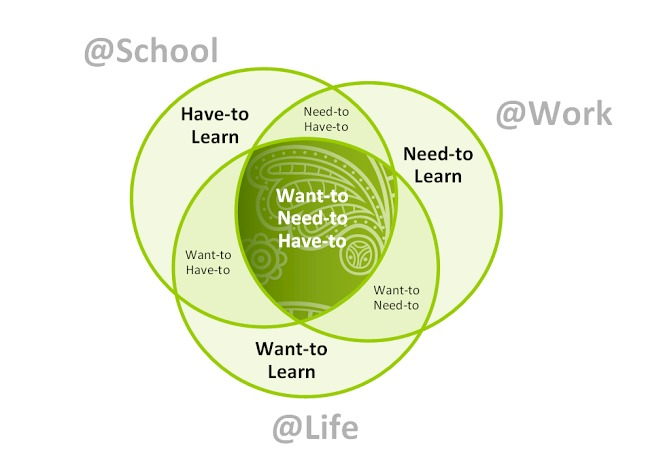
\includegraphics[width=.75\textwidth]{../pictures/learn.jpg}
\caption*{``I think because of the
tremendous changes we see in education and at work, the sets
(attitudes) are beginning to overlap more and more,'' said Joachim
Stroh of the Google+ community, Visual Metaphors.}
\end{center}
\end{figure}

Today's knowledge workers typically have instant, ubiquitous access to
the internet. The measure of their ability is an open-book exam. ``What
do you know?'' is replaced with ``What can you do?'' And if they get
bored, they can relatively easily be mentally elsewhere.

This has ramifications for the way managers manage as well as the way
teachers teach. To extract optimal performance from workers, managers
must inspire them rather than command them. Antoine de Saint-Exupéry put
it nicely: ``If you want to build a boat, do not instruct the men to saw
wood, stitch the sails, prepare the tools and organize the work, but
make them long for setting sail and travel to distant lands.''

\begin{quote}
\textbf{Jay Cross}: ``If I were an instructional designer in a moribund
training department, I'd polish up my resume and head over to marketing.
Co-learning can differentiate services, increase product usage,
strengthen customer relationships, and reduce the cost of hand-holding.
It's cheaper and more useful than advertising. But instead of just
making a copy of today's boring educational practices, build something
based on interaction and camaraderie, perhaps with some healthy
competition thrown in. Again, the emphasis should always be on learning
in order to do something!''
\end{quote}
In the section on \href{http://peeragogy.org/organize/}{organizing a
learning context}, we'll say quite a bit more about the implications
that our full conception of peer learning has for managers, teachers,
and other facilitators.
